\documentclass[a0,portrait]{a0poster}
\usepackage{multicol} % This is so we can have multiple columns of text side-by-side
\columnsep=100pt % This is the amount of white space between the columns in the poster
\columnseprule=3pt % This is the thickness of the black line between the columns in the poster

\usepackage[svgnames]{xcolor} % Specify colors by their 'svgnames', for a full list of all colors available see here: http://www.latextemplates.com/svgnames-colors
\usepackage{tcolorbox} % coloured boxing of sections
\usepackage{tikz} % manual placement of logos
\usepackage{palatino} % use the Palatino font

\usepackage{graphicx} % Required for including images
\usepackage{enumitem}
\graphicspath{{figures/}} % Location of the graphics files

\usepackage{booktabs} % Top and bottom rules for table
\usepackage[font=small,labelfont=bf]{caption} % Required for specifying captions to tables and figures

\usepackage{amsfonts, amsmath, amsthm, amssymb} % For math fonts, symbols and environments
\usepackage{wrapfig} % Allows wrapping text around tables and figures
\usepackage{mathtools}

\begin{document}

%----------------------------------------------------------------------------------------
% title and authors
\begin{minipage}[b]{0.99\linewidth}
	\begin{center}
		\veryHuge \color{DarkRed} \textbf{Reverse-engineering natural computation} \color{Black}\\ % Title
		\Huge\textit{using reaction-diffusion approaches beyond linear stability}\\[2.4cm] % Subtitle
		\huge \textbf{Gregory Sz\'ep, Luca Cardelli, Attila Csik\'asz-Nagy}\\[0.5cm]
		\vspace{1cm}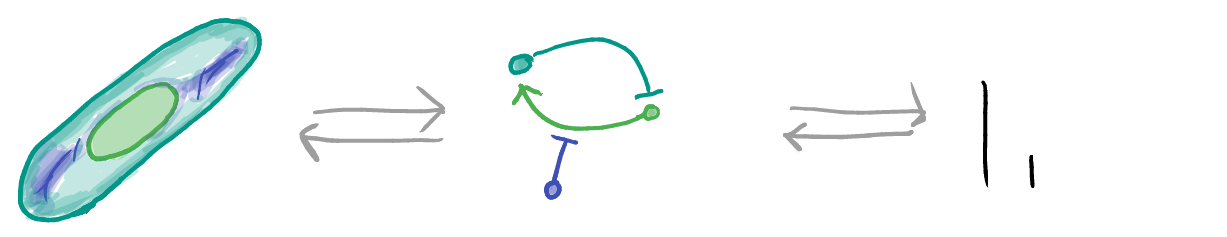
\includegraphics[width=70cm]{abstract}
		\center{mappings between levels of abstraction from biological process to algorithm}
	\end{center}
\end{minipage}

% organisation logos
{\begin{tikzpicture}[remember picture, overlay]
	\node [anchor=north west, inner sep=6cm]  at (-8,37)
		{
\includegraphics[height=7cm]{kcl}};
\end{tikzpicture}}

{\begin{tikzpicture}[remember picture, overlay]
	\node [anchor=north east, inner sep=6cm]  at (81,37)
		{
\includegraphics[height=6cm]{mrc}};
\end{tikzpicture}}

{\begin{tikzpicture}[remember picture, overlay]
	\node [anchor=south west, inner sep=6cm]  at (56,-85)
		{
\includegraphics[height=7cm]{epsrc}};
\end{tikzpicture}}
\vspace{-2cm}


% itemized thumbs up/down icons
\newcommand*\up{\item[{
\includegraphics[width=0.75em]{up}}\,\,]}
\newcommand*\down{\item[{
\includegraphics[width=0.75em]{down}}\,\,]}

%----------------------------------------------------------------------------------------
\LARGE % default text size

\begin{tcolorbox}[boxrule=2pt,arc=3.4pt,boxsep=2mm]
	\begin{center}
		\textbf{\color{Grey}Algorithm $\rightarrow$ Dynamical System \color{Black}$|$
		Given a \textit{response function} what is the \textit{minimal} reaction network?}
	\end{center}
\end{tcolorbox}

\begin{itemize}[leftmargin=5cm]
	\up Mappings between algorithms and reaction networks
	pave the path towards programming in cells \cite{Dalchau2018ComputingClocks}
	\up Dynamical structure function and Granger causality methods reconstruct networks from data
	% \up Experimentally determined response functions probe of the validity ofproposed networks \cite{Loose2011MinMinE}
	% \down Model selection is computationally expensive \cite{Mangan2017ModelCriteria} and including prior knowledge is nontrivial
	\down No general mapping exists that takes model complexity into consideration
\end{itemize}

\begin{align*}
	\partial_t\rho =
	\overbracket[2pt][10pt]{R(\rho)}^{\text{reaction}}+
	\underbracket[2pt][10pt]{S(t)}_{\text{source}}
\end{align*}

\begin{tcolorbox}[boxrule=2pt,arc=3.4pt,boxsep=2mm]
	\begin{center}
		\textbf{\color{Grey}Biological Process $\rightarrow$ System \color{Black}$|$
		What is the general routine for \textit{reducing complexity} in reaction networks?}
	\end{center}
\end{tcolorbox}

\begin{itemize}[leftmargin=5cm]
	\up Time-scale separation allows reduction of component number; introducing delays and nonlinearity
	\down There exist no dimensionality reduction and parameter relevance methods for reaction networks
\end{itemize}

\begin{tcolorbox}[boxrule=2pt,arc=3.4pt,boxsep=2mm]
	\begin{center}
		\textbf{\color{Grey}Biological Process $\rightarrow$ Dynamical System \color{Black}$|$
		How do network motifs such as \textit{switches and clocks} evolve?}
	\end{center}
\end{tcolorbox}

\begin{itemize}[leftmargin=5cm]
	\up Relationship between robustness and evolvability has been investigated \cite{Daniels2008SloppinessBiology}
	\up Sensitivity analysis has been applied to 
	\down Evolutionary relationships between different chemical networks have not been quantified
\end{itemize}

\begin{tcolorbox}[boxrule=2pt,arc=3.4pt,boxsep=2mm]
	\begin{center}
		\textbf{\color{Grey}Dynamical System \color{Black}$|$
		Given a \textit{steady state pattern} what is the \textit{minimal} reaction-diffusion network?}
	\end{center}
\end{tcolorbox}

\begin{itemize}[leftmargin=5cm]
	\up Dynamics of local equilibria show promising analysis beyond linear stability \cite{Halatek2018}
	\down Need to design attractors in phase space; no description in phase space exists
\end{itemize}

\begin{tcolorbox}[boxrule=2pt,arc=3.4pt,boxsep=2mm]
	\begin{center}
		\textbf{\color{Grey}Biological Process $\rightarrow$ Dynamical System \color{Black}$|$
		How do patterns form across \textit{growing cell populations}?}
	\end{center}
\end{tcolorbox}

\begin{itemize}[leftmargin=5cm]
	\up Differential diffusion between cytosolic, membrane and inter-cellular components give rise to patterns
	\down Finite element reaction-diffusion simulations are computationally expensive
\end{itemize}


%----------------------------------------------------------------------------------------
\vfill\normalsize

\begin{minipage}[t][][b]{0.99\textwidth}
	\bibliographystyle{style}
	\bibliography{mendeley_v2}
\end{minipage}

\end{document}
